\documentclass{standalone}
\usepackage{tikz}
\begin{document}
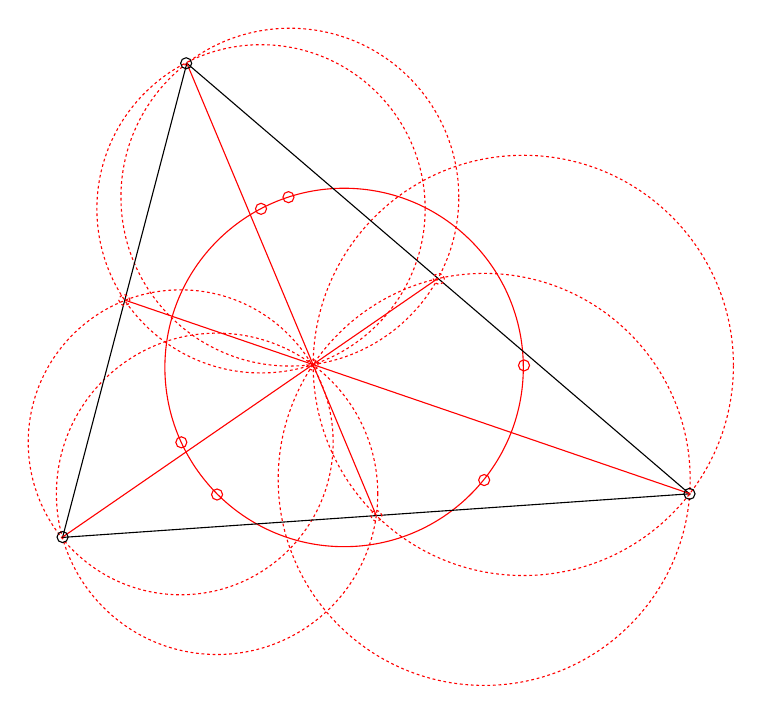
\begin{tikzpicture}[x=1pt,y=1pt]
\draw[red, dash pattern=on 1pt] (127.05,-67.49) circle (61.04);
\draw[red, dash pattern=on 1pt] (116.63,-71.71) circle (59.31);
\draw[red, dash pattern=on 1pt] (87.60,-156.08) circle (55.09);
\draw[red, dash pattern=on 1pt] (100.75,-174.69) circle (58.06);
\draw[red, dash pattern=on 1pt] (197.27,-169.48) circle (74.44);
\draw[red, dash pattern=on 1pt] (211.41,-128.29) circle (75.93);
\draw[red] (146.65,-129.03) circle (64.76);
\draw (89.83,-19.11) -- (271.46,-174.69) -- (44.92,-190.44) -- cycle;
\draw[red] (44.92,-190.32) -- (180.65,-96.77);
\draw[red] (271.71,-174.69) -- (67.50,-104.71);
\draw[red] (89.83,-19.11) -- (158.31,-182.63);
\draw[red] (116.63,-71.71) circle (2.00);
\draw[red] (126.55,-67.49) circle (2.00);
\draw[red] (211.66,-128.29) circle (2.00);
\draw[red] (197.27,-169.72) circle (2.00);
\draw[red] (100.75,-174.94) circle (2.00);
\draw[red] (87.84,-156.08) circle (2.00);
\draw[red, dash pattern=on 1pt] (67.25,-104.71) circle (2.00);
\draw[red, dash pattern=on 1pt] (180.89,-97.02) circle (2.00);
\draw[red, dash pattern=on 1pt] (158.31,-182.63) circle (2.00);
\draw (44.92,-190.32) circle (2.00);
\draw (89.58,-19.11) circle (2.00);
\draw (271.46,-174.69) circle (2.00);
\draw[red, dash pattern=on 1pt] (135.24,-128.04) circle (2.00);
\end{tikzpicture}
\end{document}
